\section{Generative modeling 2}
\subsection{Dimensionality reduction}
Can serve as a preprocessing step to help improve results and increase speed.
Allows fro visual exploration of data and possible science discovery.
\subsubsection{Principle Components Analysos (PCA)}
PCA prioritizes the maximization of the data's variance in the embedding at the expense of local structure

Principle components are the Eigenvectors of the convariance Matrix.
Neglects the preservation of local detail.
\subsubsection{t-SNE}
\begin{figure}[!h]
    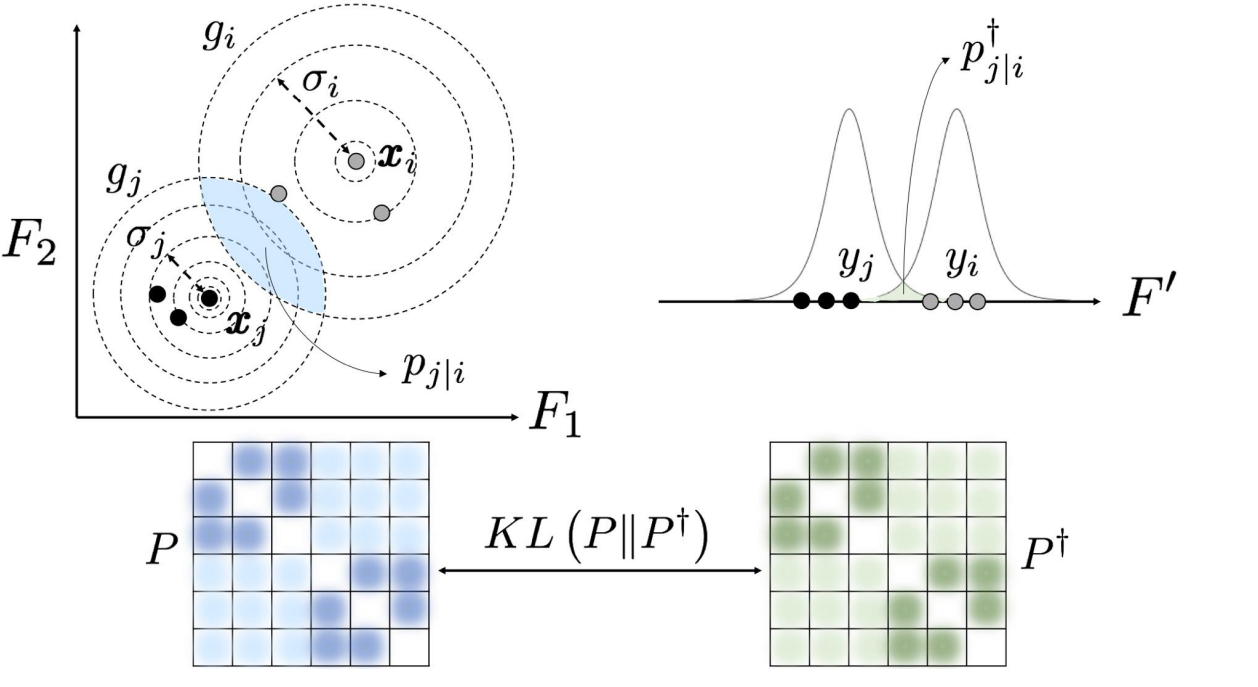
\includegraphics[width = \columnwidth]{figures/GenAI2/tSNETheory.png}
\end{figure}
\begin{itemize}
    \item Prior: Random position of n-points in 1D
    \item Loss: KL-divergence between statistical matrices.
    \item Optimization: Gradient descent + incrementally shifting 1D points
    \item Hyperparameters: perplexity
\end{itemize}

\subsubsection{Interpretation}
Playing with preplexity: Low perplexity preserves local structure, high preplexity preserves global structure, if preplexity exceeds the number of points in the dataset we get strange behaviour that should not be trusted.

Playing with convergence time and fixed perplexity: must wait until updates are relatively small. First four panels have not properly converged. If you see strange pinched shapes be cautions. Generally takes 5000 iterations.


Interpretation caution:
\begin{itemize}
    \item  Cluster sizes might not mean anything.
    \item Distance between clusters might not mean anything
    \item Random noise doesn't always look random
    \item You can see some shapes sometimes
    \item To derive topological insights you have to test many perplexities
\end{itemize}

\subsection{Variational Autoencoder (VAE)}
VAE is 
\begin{itemize}
    \item Quick for sampling
    \item Easy to train
    \item Produces blurry images
\end{itemize}

\subsubsection{Autoencoder}
\begin{itemize}
    \item Neural network trained to reproduce its input x
    \item No labels needed, unsupervised training
    \item Discover patterns in the input space and encoding them in latent space
\end{itemize}
\begin{figure}[!h]
     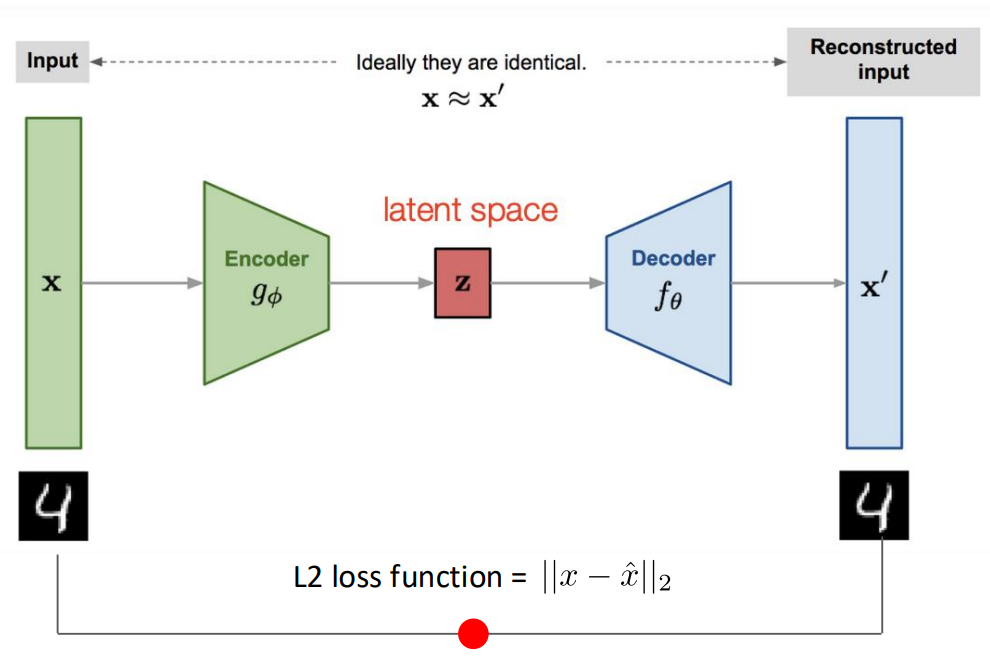
\includegraphics[width = \columnwidth]{figures/GenAI2/Autoencoder.png}
\end{figure}

Need to restrict model to learn interesting representations.
Therefore \(\text{dim}(z) < \text{dim}(x)\).

If \(\text{dim}(z) = \text{dim}(x)\) then the network would simply learn th identity matrix
 

